\section{Punto 1}
\textit{Describir las ventajas y desventajas con respecto a las implementaciones estática y dinámica de un grafo, considerando las operaciones principales como inserción y eliminación de vértices y arcos, recorridos, etc.}\\

\textbf{Implementación estática: }Un ejemplo de representación estática sencilla para grafos es la matriz de adyacencia, esta consiste en una matriz M de tamaño $N \times N$ de tipo boolean en la cual se puede representar un grafo de N vertices. Si se trata de un grafo dirigido, la celda M[i,j] indica si existe un arco entre el vertice i y el vértice j. Si existe un arco (i,j), la celda esta en true y false en caso contrario. En caso de utilizarse para modelar un grafo no dirigido, para una arista (i,j) se inicializan a true ambas celdas M[i,j] y M[j,i]. por lo que la matriz sera simétrica. En la figura \ref{fig:MatrizAdyacencia} se muestra un ejemplo de un grafo no etiquetado representado con una matriz de adyacencia.

\begin{figure}[!htb]
  \centering
  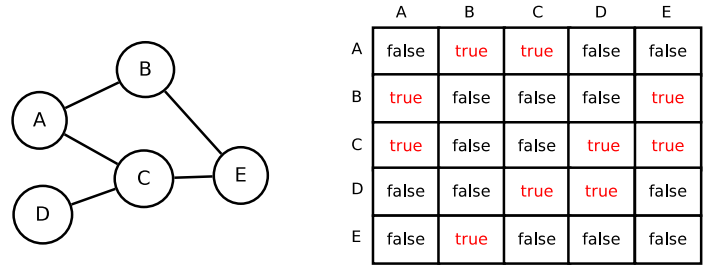
\includegraphics[width=\textwidth, scale=1]{Images/Punto1/MatrizAdyacencia.png}
  \caption{Representación de grafo no etiquetado con matriz de adyacencia}
  \label{fig:MatrizAdyacencia}
\end{figure}

Este tipo de representación tiene la ventaja del acceso de $O(1)$ a cualquier arco del grafo. Por lo general, es la representación mas adecuada cuando los vertices son del tipo de los indices del arreglo, pero resulta poco practica cuando se necesita almacenar vertices de otro tipo. A medida que las celdas de la matriz tengan mas valores false (es decir que tiene pocos arcos entre los vertices), la matriz ocupara mas espacio del necesario. Las matrices que tienen $30\%$ o menos de sus celdas en valores distintos de vació, se llaman ralas y siempre se recomienda utilizar una implementación alternativa para estas. Como suele ocurrir con las implementaciones estáticas, tiene la desventaja de ocupar mas espacio de memoria del que generalmente se necesita.\\


\textbf{Implementación dinamica: }Un ejemplo son las listas de adyacencia donde se definen nodos vertices, uno por cada vértice del grafo, que se entrelazan entre ellos formando una lista. Ademas se definen los denominados nodos adyacentes que se enlazan a los nodos vertices conformando una lista que representa todos los vertices adyacentes de un determinado vértice, en la figura \ref{fig:ListaAdyacencia} se puede ver un ejemplo para un digrafo no etiquetado

\begin{figure}[!htb]
  \centering
  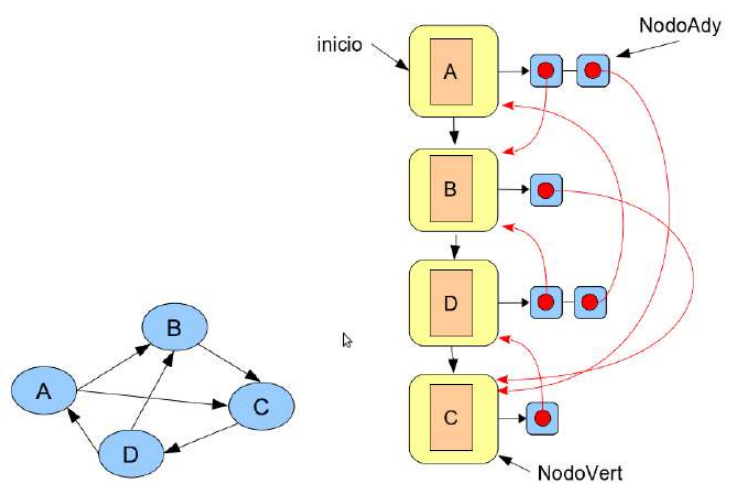
\includegraphics[width=\textwidth, scale=1]{Images/Punto1/ListaAdyacencia.png}
  \caption{Representación de grafo no etiquetado con listas de adyacencia}
  \label{fig:ListaAdyacencia}
\end{figure}

En esta representación se pueden destacar las siguientes características: 
\begin{itemize}
  \item La implementación es similar para vertices de cualquier tipo (a diferencia de la implementación estática que, al menos en java, solo seria eficiente para vertices de tipo entero $\geq 0$)
  \item La cantidad de vertices puede crecer y decrecer durante la ejecución, simplemente agregando un nuevo nodo a la lista de vertices
  \item La lista de nodos adyacentes de cada vértice también puede crecer o decrecer como sea necesario, aunque en este caso a mayor cantidad de adyacentes menor eficiencia para recorrer el grafo y realizar las operaciones correspondientes
\end{itemize}